\documentclass[10pt]{beamer}
\usepackage[english]{babel}
\usepackage[utf8]{inputenc}
\usepackage[T1]{fontenc}
\usepackage{helvet}

%-------------------------------------------------------
% INFORMATION IN THE TITLE PAGE
%-------------------------------------------------------

\newcommand{\cstitle}{\textbf{Detección de neo antígenos\\utilizando \textit{deep learning}}}
\subtitle[]{CPO}
\newcommand{\cscourseCode}{Matemáticas discretas II}
\newcommand{\csauthor}{PhD(c). Vicente Machaca Arceda}
\institute[UNSA]{Universidad de Ingeniería y Tecnología}
\newcommand{\csemail}{vmachaca@utec.edu.pe}
\newcommand{\instituteabr}{UTEC}
\newcommand{\nameUp}{}
\date{2022-I}
\title[\cscourseCode]{\cstitle}
\author{\csauthor}
%%%%%%%%%%%%%%%%%

%-------------------------------------------------------
% CHOOSE THE THEME
%-------------------------------------------------------
\def\mycmd{0} % UNSA
\def\mycmd{1} % SALLE
\def\mycmd{2} % UTEC
%-------------------------------------------------------

\if\mycmd0
\usepackage{csformat}
\newcommand{\chref}[3][blue]{\href{#2}{\color{#1}{#3}}}%

\fi

\if\mycmd1
\usetheme[]{Feather}
\newcommand{\chref}[2]{	\href{#1}{{\usebeamercolor[bg]{Feather}#2}} }
\fi

\if\mycmd2
\usetheme{UTEC2020}	
\newcommand{\chref}[3][blue]{\href{#2}{\color{#1}{#3}}}%
\fi

\newcommand{\1}{
	\setbeamertemplate{background}{
		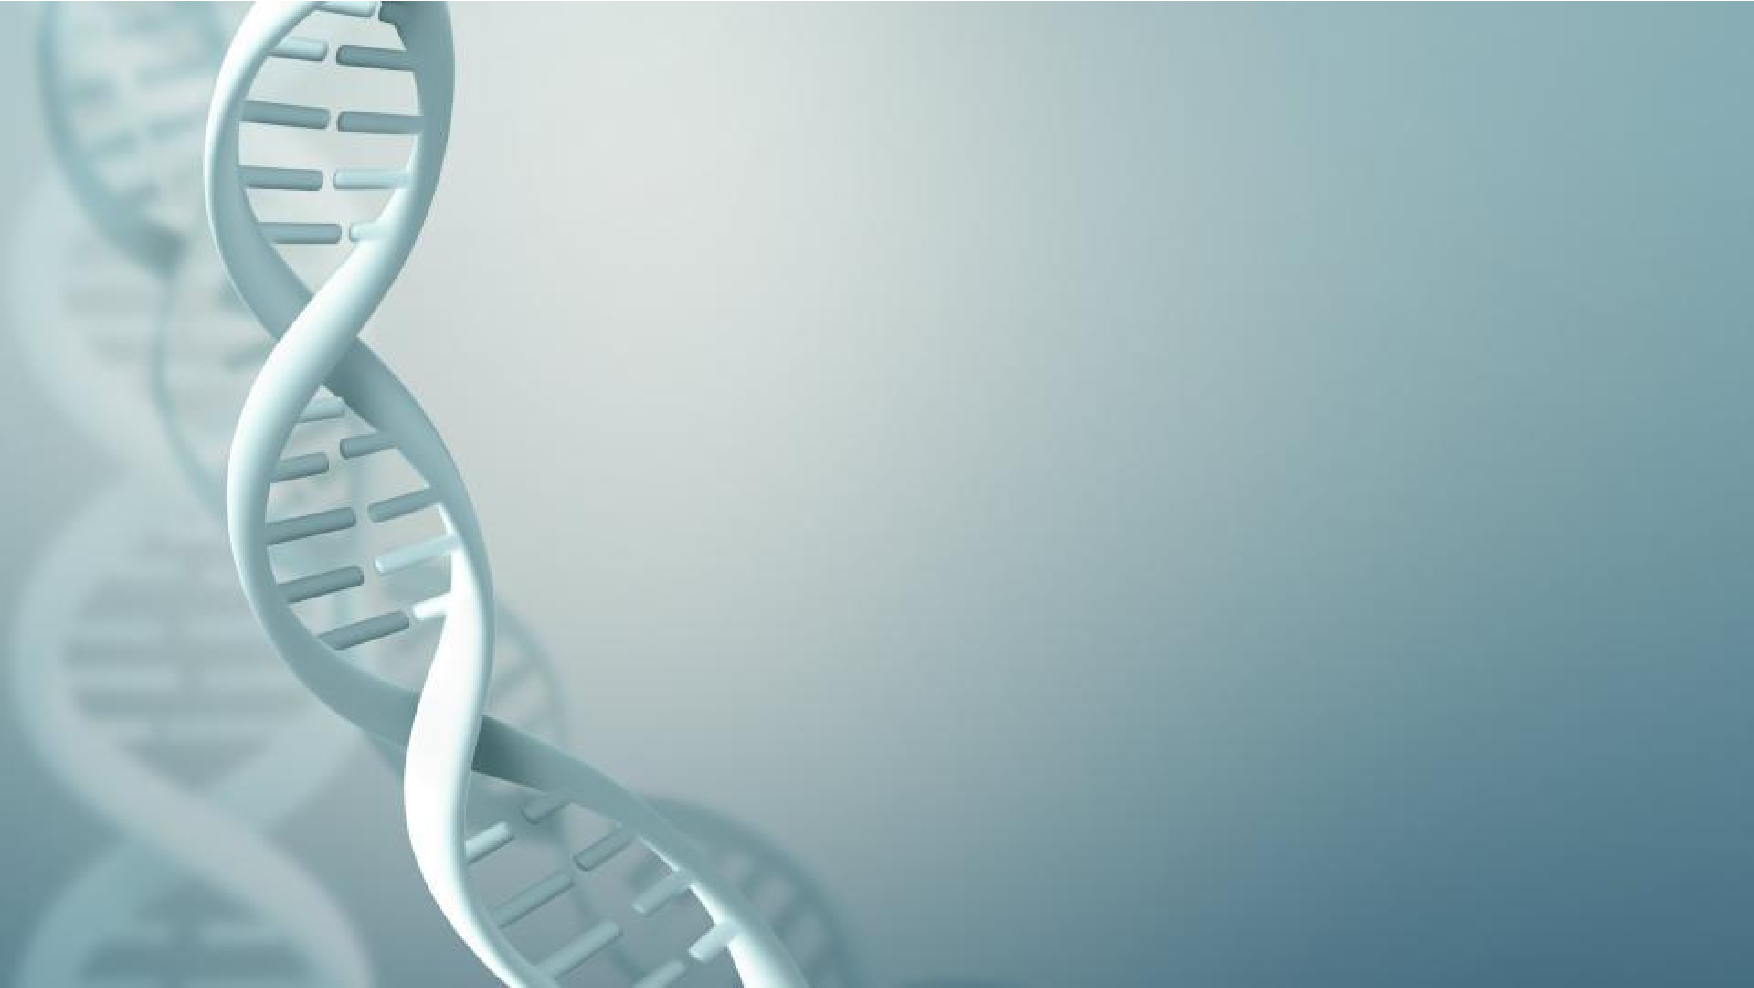
\includegraphics[width=\paperwidth,height=\paperheight]{img/1}
		\tikz[overlay] \fill[fill opacity=0.75,fill=white] (0,0) rectangle (-\paperwidth,\paperheight);
	}
}



%-------------------------------------------------------
% THE BODY OF THE PRESENTATION
%-------------------------------------------------------

\begin{document}
	
	
	\AtBeginSection[]
	{
		\begin{frame}
			\frametitle{Contenido}
			\tableofcontents[currentsubsection]
		\end{frame}
	}
	
	
	%-------------------------------------------------------
	% THE TITLEPAGE
	%-------------------------------------------------------
	
	\if\mycmd0
	\maketitle
	\fi
	
	\if\mycmd1 % MY THEME
	\1{
		\begin{frame}[plain,noframenumbering] 
			\titlepage 
	\end{frame}}
	\fi
	
	\if\mycmd2
	\begin{frame}
		\titlepage
	\end{frame}
	\fi
	%-------------------------------------------------------
	%-------------------------------------------------------


%-------------------------------------------------------
%-------------------------------------------------------
\begin{frame}{Contenido}
	\tableofcontents
\end{frame}
%-------------------------------------------------------
%-------------------------------------------------------

%-------------------------------------------------------
%-------------------------------------------------------
\begin{frame}{Presentación}{}
	\begin{itemize}
		\item PhD(c). Vicente Enrique Machaca Arceda. 
		\item Profesor UTEC (TP).
		\item Investigador en Bioinformática y Aprendizaje de Maquina.	
		\item \chref{https://scholar.google.com/citations?user=Y2taS2MAAAAJ&hl=es&oi=ao}{Index-h 5}.  	
	\end{itemize}
\end{frame}
%-------------------------------------------------------
%-------------------------------------------------------

%-------------------------------------------------------
%-------------------------------------------------------
\begin{frame}{Presentación}{Publicaciones}
	\begin{table}[]
		\setlength{\tabcolsep}{0.5em} % for the horizontal padding
		{\renewcommand{\arraystretch}{1.4}% for the vertical padding
			\begin{tabular}{llp{7cm}}
				\textbf{Year} & \textbf{Country} & \textbf{Title}                                                                                                              \\
				\hline
				2020          & USA              & Small Ship Detection on Optical Satellite Imagery with YOLO and YOLT                                                        \\
				2018          & Brasil           & Fast Car Crash Detection in Video                                                                                           \\
				2016          & Chile            & Fast Face Detection in Violent Video Scenes                                                                                 \\
				2016          & Costa Rica       & Real Time Violence Detection in Video with ViF and Horn-Schunck                                                             \\
				2016          & Costa Rica       & Optimization model for face detection in video sequences                                                                    \\
				2015          & Chile            & Real Time Violence Detection in Video                                                                                      
			\end{tabular}
		}
	\end{table}
\end{frame}
%-------------------------------------------------------
%-------------------------------------------------------

%-------------------------------------------------------
%-------------------------------------------------------
\begin{frame}{Presentation}{Publications}
	\begin{table}[]
		\setlength{\tabcolsep}{0.5em} % for the horizontal padding
		{\renewcommand{\arraystretch}{1.4}% for the vertical padding
			\begin{tabular}{llp{7cm}}
				\textbf{Year} & \textbf{Country} & \textbf{Title}                                                                                                              \\
				\hline
				2022          &  USA                & ArgosMol: A Web Tool for Protein Structure Prediction and Visualization             \\
				2021          &  Chapter                & COVID-19 Pandemic: Analysis and Statistics of Confirmed Cases             \\
				2020          &  Canada          & An Analysis of k-Mer Frequency Features with Machine Learning Models for Viral Subtyping of Polyomavirus and HIV-1 Genomes                                                        \\
				
				2020          & Canada           & An analysis of k-mer frequency features with SVM and CNN for viral subtyping classification \\
				2020          & Canada           & Forecasting time series with Multiplicative Trend Exponential Smoothing and LSTM: COVID-19 case study                       \\
				
				
			\end{tabular}
		}
	\end{table}
\end{frame}
%-------------------------------------------------------
%-------------------------------------------------------


%%%%%%%%%%%%%%%%%%%%%%%%%%%%%%%%%%%%%%%%%%%%%%%%%%%%%%%%%%%%%%%%%%%%%%%%%%%%%%%%%%%%%%%%%%%%%%%%%%%%%%%%%%%%%%%%
%%%%%%%%%%%%%%%%%%%%%%%%%%%%%%%%%%%%%%%%%%%%%%%%%%%%%%%%%%%%%%%%%%%%%%%%%%%%%%%%%%%%%%%%%%%%%%%%%%%%%%%%%%%%%%%%
%%%%%%%%%%%%%%%%%%%%%%%%%%%%%%%%%%%%%%%%%%%%%%%%%%%%%%%%%%%%%%%%%%%%%%%%%%%%%%%%%%%%%%%%%%%%%%%%%%%%%%%%%%%%%%%%
\section{Marco teórico}
%%%%%%%%%%%%%%%%%%%%%%%%%%%%%%%%%%%%%%%%%%%%%%%%%%%%%%%%%%%%%%%%%%%%%%%%%%%%%%%%%%%%%%%%%%%%%%%%%%%%%%%%%%%%%%%%
%%%%%%%%%%%%%%%%%%%%%%%%%%%%%%%%%%%%%%%%%%%%%%%%%%%%%%%%%%%%%%%%%%%%%%%%%%%%%%%%%%%%%%%%%%%%%%%%%%%%%%%%%%%%%%%%
%%%%%%%%%%%%%%%%%%%%%%%%%%%%%%%%%%%%%%%%%%%%%%%%%%%%%%%%%%%%%%%%%%%%%%%%%%%%%%%%%%%%%%%%%%%%%%%%%%%%%%%%%%%%%%%%

%%%%%%%%%%%%%%%%%%%%%%%%%%%%%%%%%%%%%%%%%%%%%%%%%%%%%%%%%%%%%%%%%%%%%%%%%%%%%%%%%%%%%%%%%%%%%%%%%%%%%%%%%%%%%%%%
%%%%%%%%%%%%%%%%%%%%%%%%%%%%%%%%%%%%%%%%%%%%%%%%%%%%%%%%%%%%%%%%%%%%%%%%%%%%%%%%%%%%%%%%%%%%%%%%%%%%%%%%%%%%%%%%
%%%%%%%%%%%%%%%%%%%%%%%%%%%%%%%%%%%%%%%%%%%%%%%%%%%%%%%%%%%%%%%%%%%%%%%%%%%%%%%%%%%%%%%%%%%%%%%%%%%%%%%%%%%%%%%%
\subsection{Bioinformática y DNA}
%%%%%%%%%%%%%%%%%%%%%%%%%%%%%%%%%%%%%%%%%%%%%%%%%%%%%%%%%%%%%%%%%%%%%%%%%%%%%%%%%%%%%%%%%%%%%%%%%%%%%%%%%%%%%%%%
%%%%%%%%%%%%%%%%%%%%%%%%%%%%%%%%%%%%%%%%%%%%%%%%%%%%%%%%%%%%%%%%%%%%%%%%%%%%%%%%%%%%%%%%%%%%%%%%%%%%%%%%%%%%%%%%
%%%%%%%%%%%%%%%%%%%%%%%%%%%%%%%%%%%%%%%%%%%%%%%%%%%%%%%%%%%%%%%%%%%%%%%%%%%%%%%%%%%%%%%%%%%%%%%%%%%%%%%%%%%%%%%%

%-------------------------------------------------------
%-------------------------------------------------------
\begin{frame}{Bioinformática}{}		
	\begin{figure}
		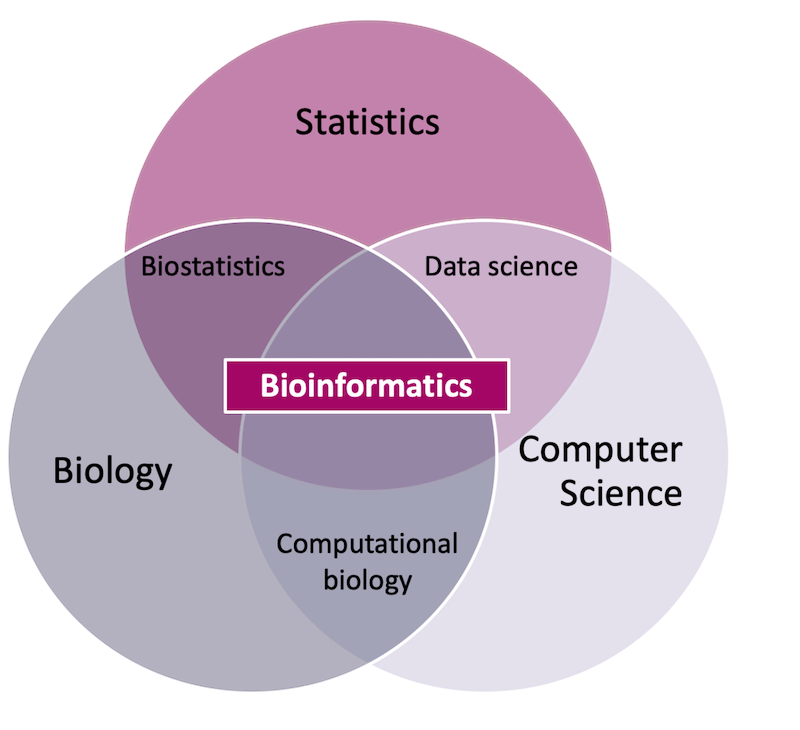
\includegraphics[width=0.7\textwidth]{img/neoantigen/bioinformatics2}
		
	\end{figure}		
\end{frame}
%-------------------------------------------------------
%-------------------------------------------------------

%-------------------------------------------------------
%-------------------------------------------------------
\begin{frame}{Bioinformática}{}		
	\begin{figure}
		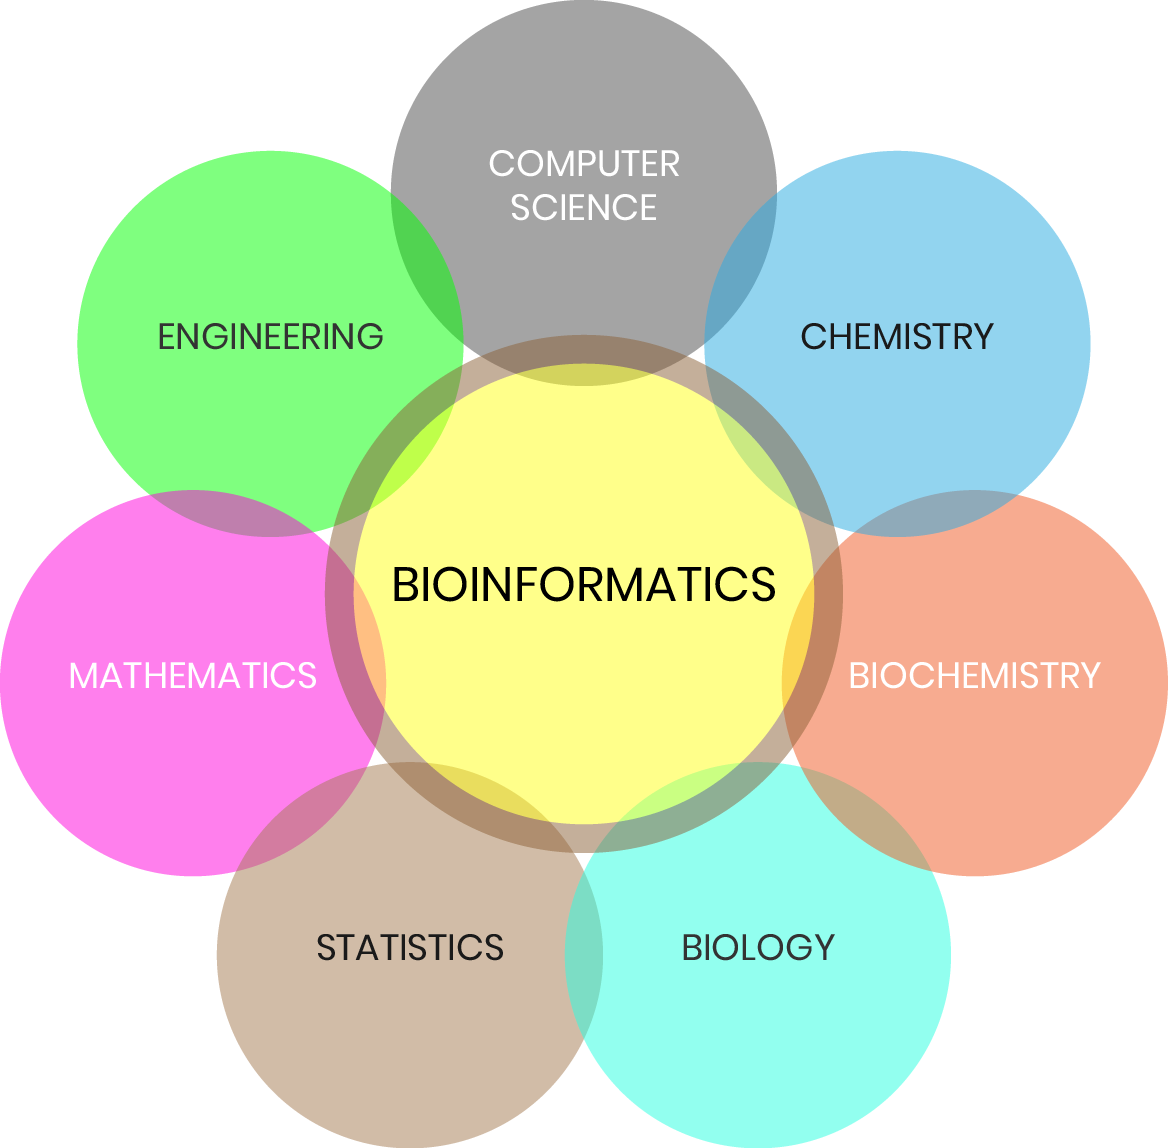
\includegraphics[width=0.6\textwidth]{img/neoantigen/bioinformatics}
		
	\end{figure}		
\end{frame}
%-------------------------------------------------------
%-------------------------------------------------------

%-------------------------------------------------------
%-------------------------------------------------------
\begin{frame}{DNA}{Localización}
	\begin{figure}[]
		\centering
		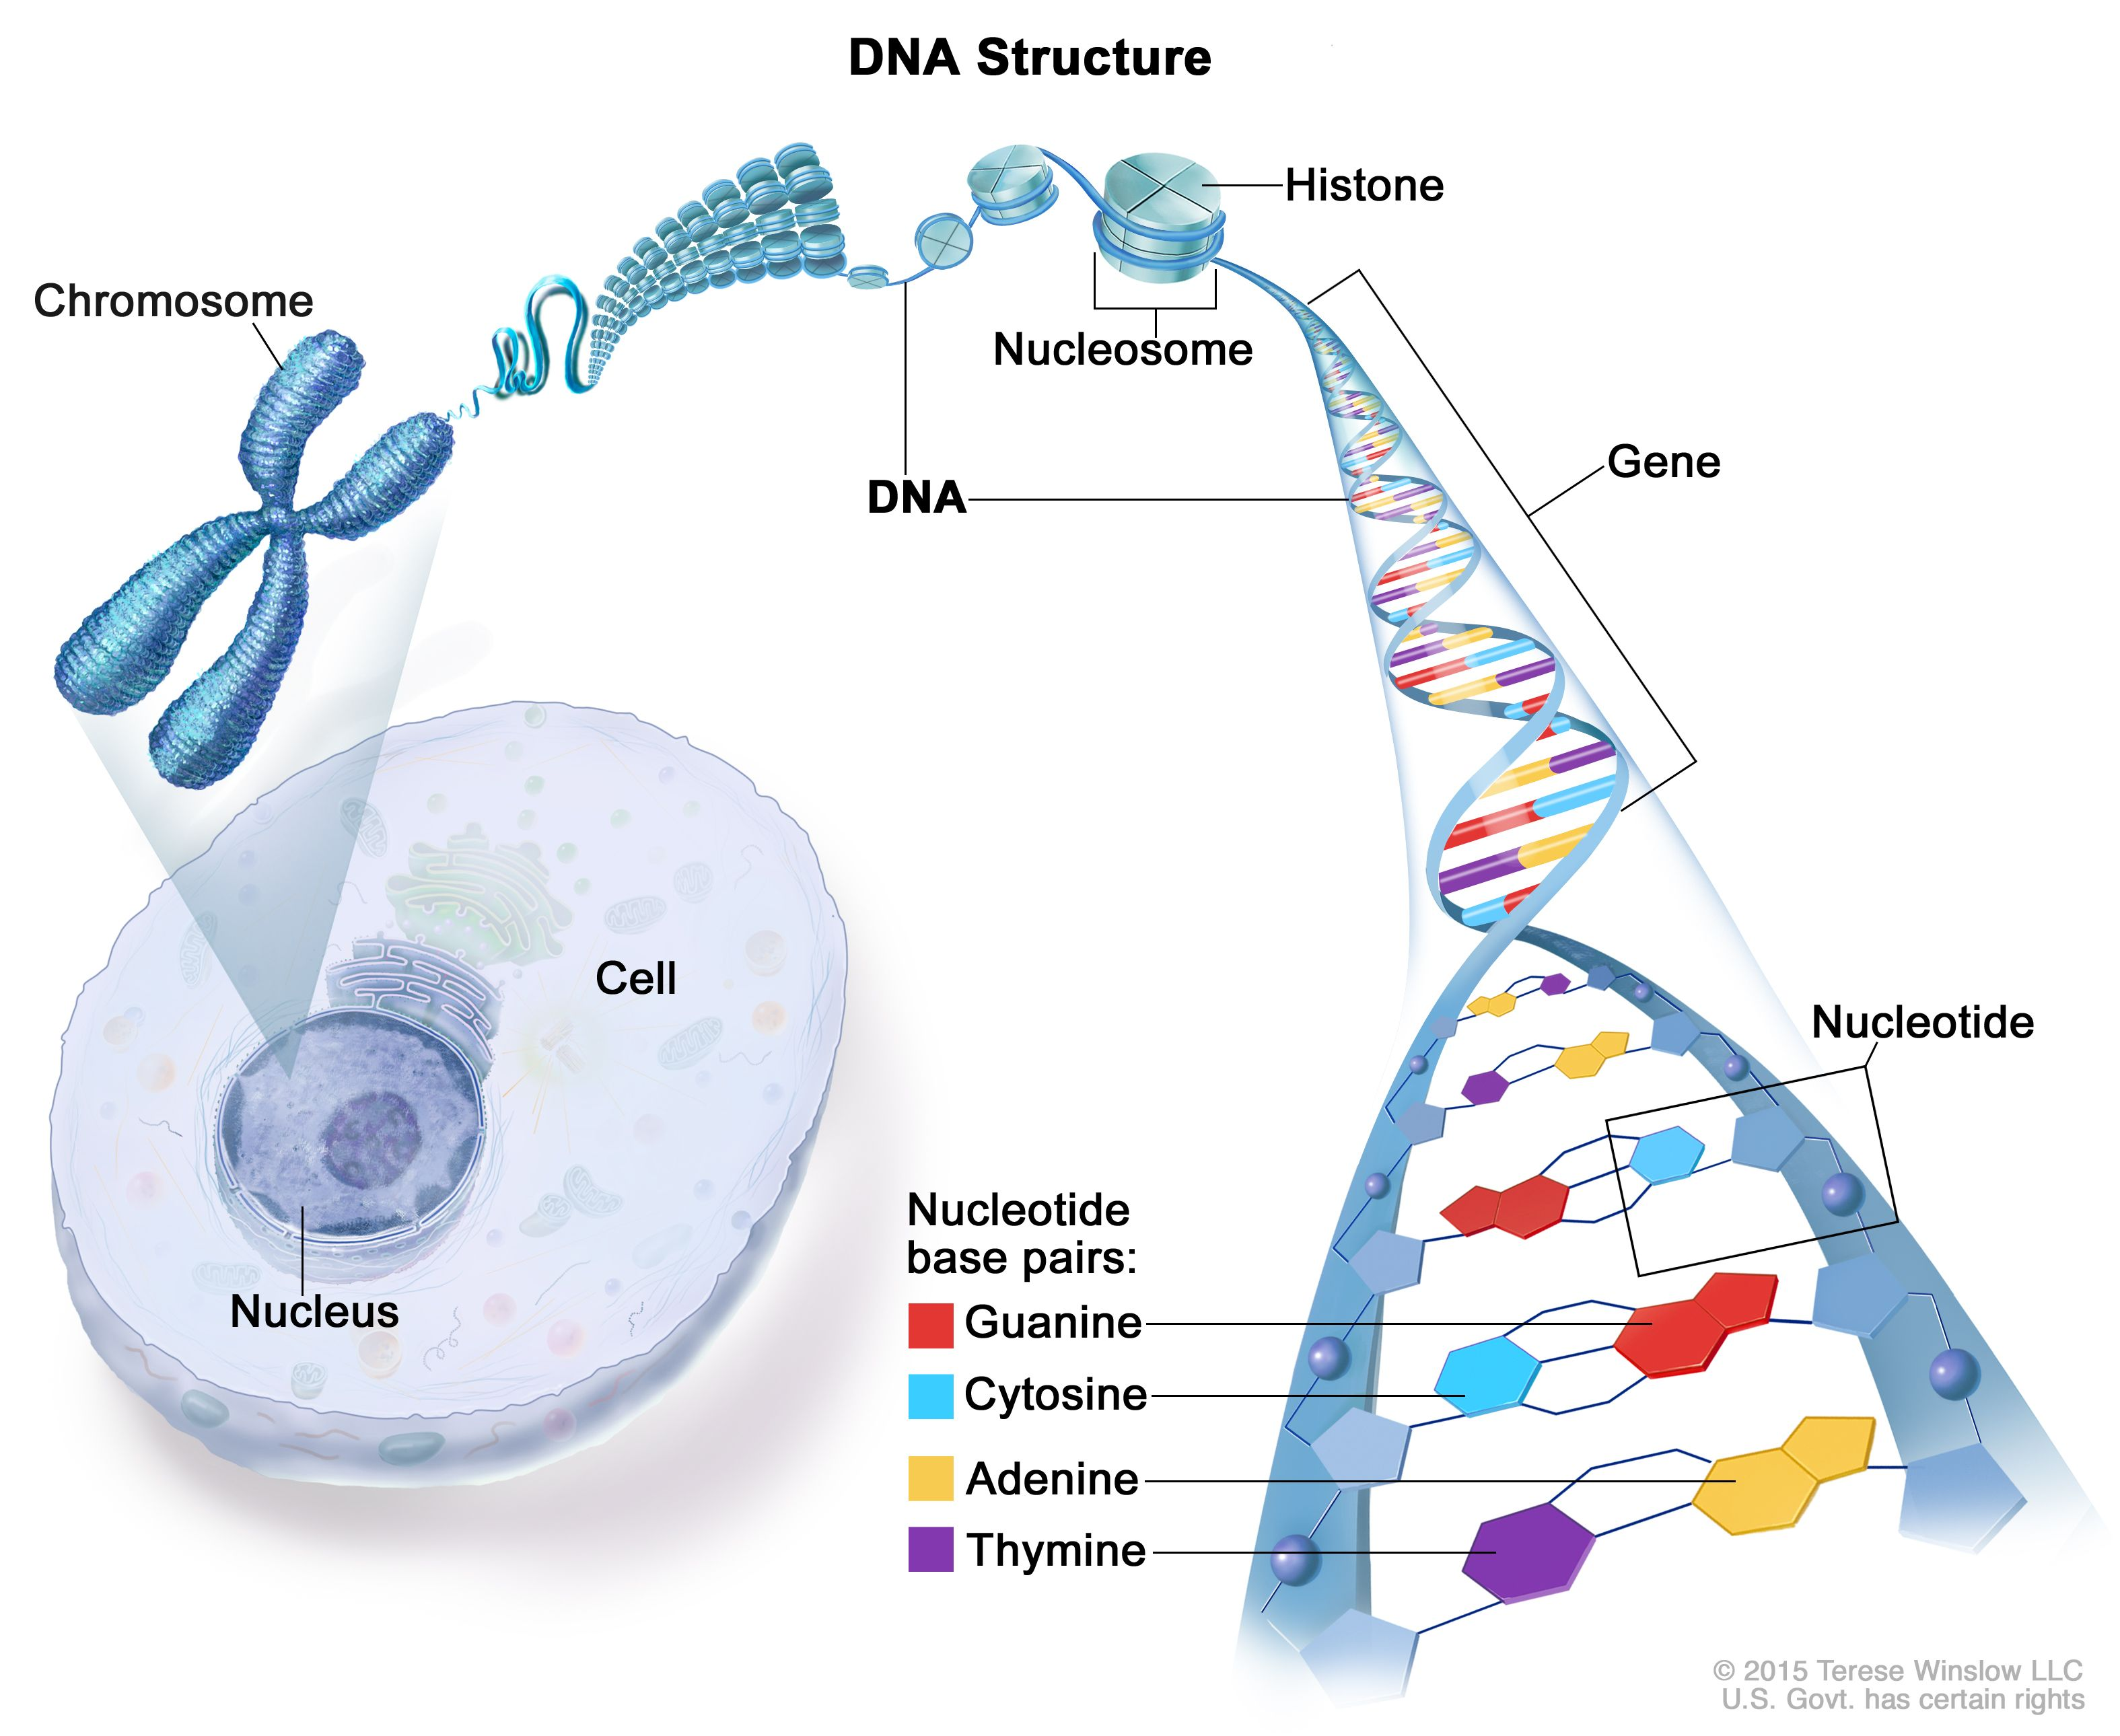
\includegraphics[width=\textwidth,height=0.65\textheight,keepaspectratio]{img/neoantigen/dna}
		\label{img:mot2}
		\caption{Where DNA is located \cite{NCIdictionary2022}.}
	\end{figure}
\end{frame}
%-------------------------------------------------------
%-------------------------------------------------------



%-------------------------------------------------------
%-------------------------------------------------------
\begin{frame}{DNA}{De DNA a proteínas}
	\begin{figure}[]
		\centering
		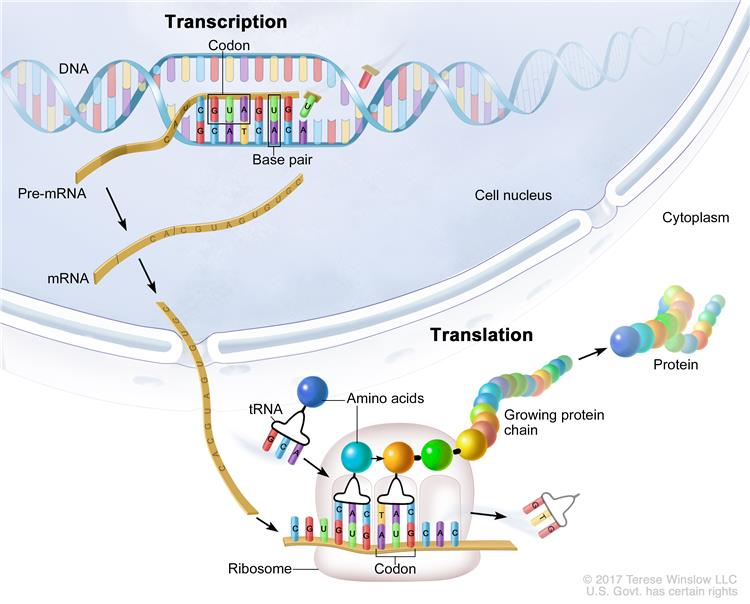
\includegraphics[width=0.7\textwidth]{img/neoantigen/trans.jpg}
		\caption{Transcription and translation \cite{nci2020}.}
	\end{figure}
\end{frame}
%-------------------------------------------------------
%-------------------------------------------------------

%%%%%%%%%%%%%%%%%%%%%%%%%%%%%%%%%%%%%%%%%%%%%%%%%%%%%%%%%%%%%%%%%%%%%%%%%%%%%%%%%%%%%%%%%%%%%%%%%%%%%%%%%%%%%%%%
%%%%%%%%%%%%%%%%%%%%%%%%%%%%%%%%%%%%%%%%%%%%%%%%%%%%%%%%%%%%%%%%%%%%%%%%%%%%%%%%%%%%%%%%%%%%%%%%%%%%%%%%%%%%%%%%
%%%%%%%%%%%%%%%%%%%%%%%%%%%%%%%%%%%%%%%%%%%%%%%%%%%%%%%%%%%%%%%%%%%%%%%%%%%%%%%%%%%%%%%%%%%%%%%%%%%%%%%%%%%%%%%%
\subsection{Mutaciones}
%%%%%%%%%%%%%%%%%%%%%%%%%%%%%%%%%%%%%%%%%%%%%%%%%%%%%%%%%%%%%%%%%%%%%%%%%%%%%%%%%%%%%%%%%%%%%%%%%%%%%%%%%%%%%%%%
%%%%%%%%%%%%%%%%%%%%%%%%%%%%%%%%%%%%%%%%%%%%%%%%%%%%%%%%%%%%%%%%%%%%%%%%%%%%%%%%%%%%%%%%%%%%%%%%%%%%%%%%%%%%%%%%
%%%%%%%%%%%%%%%%%%%%%%%%%%%%%%%%%%%%%%%%%%%%%%%%%%%%%%%%%%%%%%%%%%%%%%%%%%%%%%%%%%%%%%%%%%%%%%%%%%%%%%%%%%%%%%%%

%-------------------------------------------------------
%-------------------------------------------------------
\begin{frame}{Variantes y Mutaciones}{Tipos}
	\begin{block}{}
		\begin{itemize}
			\item \textbf{\textit{Single-Nucleotide Variant} (SNV)}, cambios a menos de 10 bases.
			\item \textbf{\textit{Structural Variation} (SV)}, cambios a mas de 10 bases, incluso pueden llegar a aumentar la cantidad de cromosomas.
		\end{itemize}	
	\end{block}
\end{frame}
%-------------------------------------------------------
%-------------------------------------------------------

%-------------------------------------------------------
%-------------------------------------------------------
\begin{frame}{Variantes y Mutaciones}{Ejemplo}
	\begin{figure}[]
		\centering
		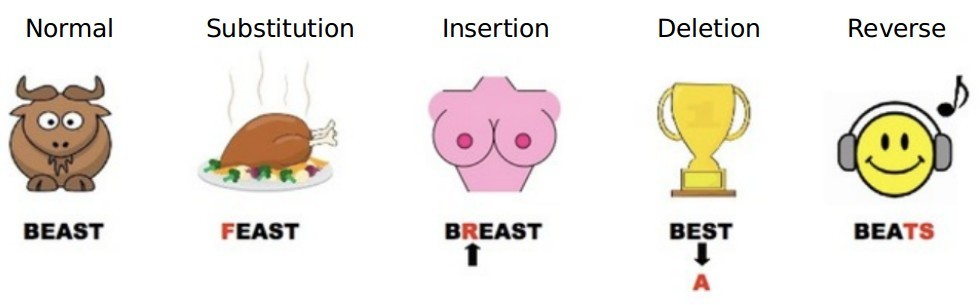
\includegraphics[width=\textwidth,height=0.7\textheight,keepaspectratio]{img/neoantigen/point_mutations_med.jpg}
		\label{img:alig}
		\caption{Overview of the Different Types of Point Mutations.}
	\end{figure}
\end{frame}
%-------------------------------------------------------
%-------------------------------------------------------

%-------------------------------------------------------
%-------------------------------------------------------
\begin{frame}{Variantes y Mutaciones}{}
	\begin{figure}[h]
		\centering
		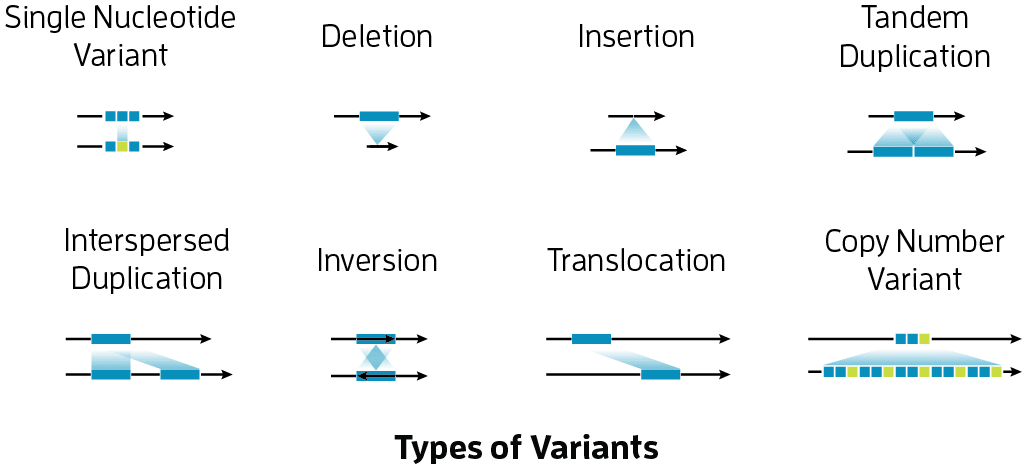
\includegraphics[width=\textwidth]{img/neoantigen/variants}
		\caption{Example of structural variants. Source: \cite{sv_pacbio_2021}}
		\label{fig:variants}
	\end{figure}	
\end{frame}
%-------------------------------------------------------
%-------------------------------------------------------

%-------------------------------------------------------
%-------------------------------------------------------
\begin{frame}{Variantes y Mutaciones}{\textit{Frameshift}}
	\begin{figure}[]
		\centering
		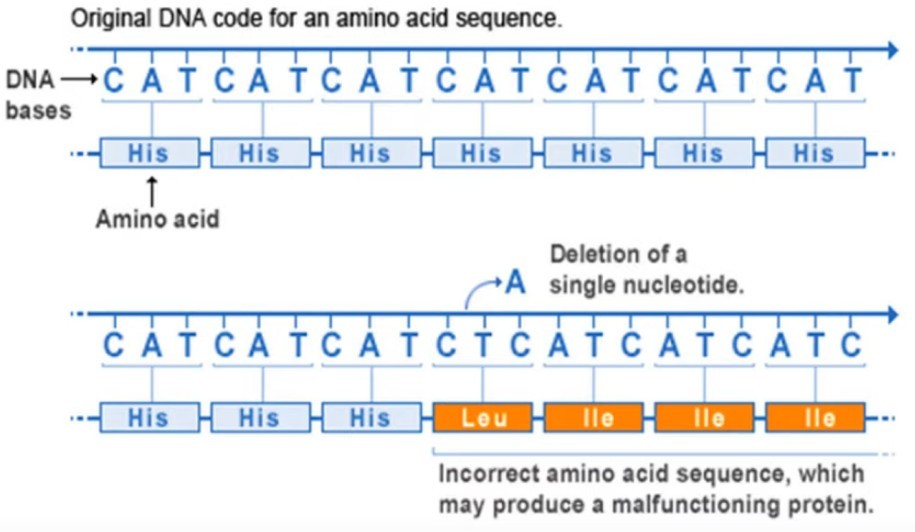
\includegraphics[width=\textwidth,height=0.6\textheight,keepaspectratio]{img/neoantigen/mut.jpg}
		\caption{Ejemplo de una mutación INDELS causante de un \textit{frameshift}.}
	\end{figure}
\end{frame}
%-------------------------------------------------------
%-------------------------------------------------------

%-------------------------------------------------------
%-------------------------------------------------------
\begin{frame}{Variantes y Mutaciones}{\textit{Frameshift}}
	\begin{block}{}
		Los \textit{Frameshift variants} estan muy relacionados a la enfermedad Tay–Sachs  (destrucción de células nerviosas). Tambien, incrementa la susceptibilidad a varios tipos de Cáncer \cite{zimmerman1997inherited, xu2018review}.
	\end{block}	
\end{frame}
%-------------------------------------------------------
%-------------------------------------------------------

%-------------------------------------------------------
%-------------------------------------------------------
\begin{frame}{Fusión de genes}{}
	\begin{figure}[h]
		\centering
		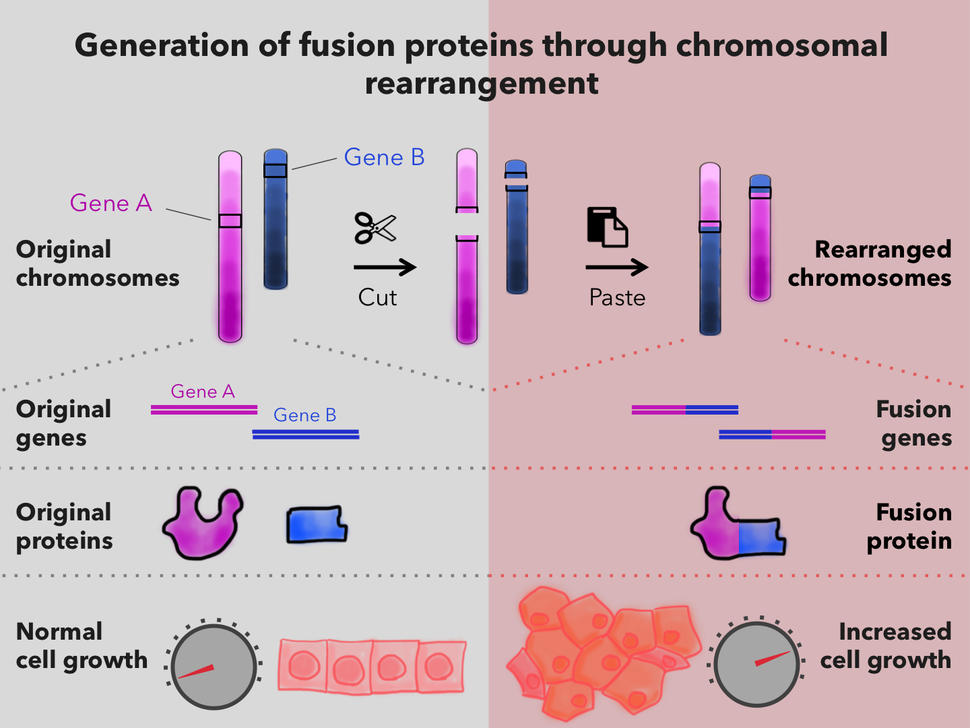
\includegraphics[width=0.8\textwidth]{img/neoantigen/gene_fusion_1}
		\caption{Ejemplo de una fución de genes.}
		\label{fig:cnv}
	\end{figure}	
\end{frame}
%-------------------------------------------------------
%-------------------------------------------------------


%-------------------------------------------------------
%-------------------------------------------------------
\begin{frame}{Variaciones a nivel de cromosomas}{}
	\begin{figure}
		\centering
		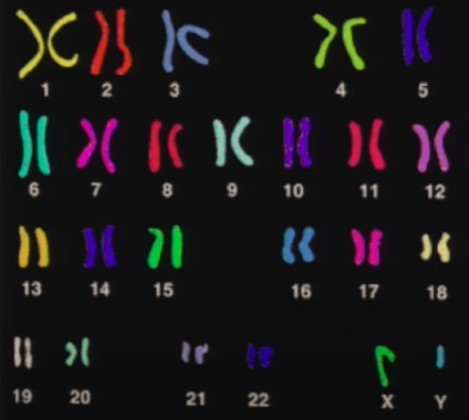
\includegraphics[width=0.6\textwidth]{img/neoantigen/chrom}
		\caption{Los 46 cromosomas presentes en una célula.}
	\end{figure}		
\end{frame}
%-------------------------------------------------------
%-------------------------------------------------------

%-------------------------------------------------------
%-------------------------------------------------------
\begin{frame}{Variaciones a nivel de cromosomas}{}
	\begin{figure}
		\centering
		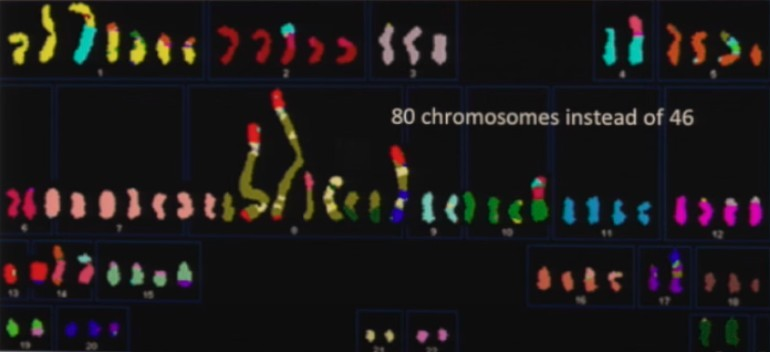
\includegraphics[width=\textwidth]{img/neoantigen/chrom3}
		\caption{Cromosomas de una mujer con Cáncer de mama (1971).}
	\end{figure}		
\end{frame}
%-------------------------------------------------------
%-------------------------------------------------------

%%%%%%%%%%%%%%%%%%%%%%%%%%%%%%%%%%%%%%%%%%%%%%%%%%%%%%%%%%%%%%%%%%%%%%%%%%%%%%%%%%%%%%%%%%%%%%%%%%%%%%%%%%%%%%%%
%%%%%%%%%%%%%%%%%%%%%%%%%%%%%%%%%%%%%%%%%%%%%%%%%%%%%%%%%%%%%%%%%%%%%%%%%%%%%%%%%%%%%%%%%%%%%%%%%%%%%%%%%%%%%%%%
%%%%%%%%%%%%%%%%%%%%%%%%%%%%%%%%%%%%%%%%%%%%%%%%%%%%%%%%%%%%%%%%%%%%%%%%%%%%%%%%%%%%%%%%%%%%%%%%%%%%%%%%%%%%%%%%
\subsection{Neo antígenos}
%%%%%%%%%%%%%%%%%%%%%%%%%%%%%%%%%%%%%%%%%%%%%%%%%%%%%%%%%%%%%%%%%%%%%%%%%%%%%%%%%%%%%%%%%%%%%%%%%%%%%%%%%%%%%%%%
%%%%%%%%%%%%%%%%%%%%%%%%%%%%%%%%%%%%%%%%%%%%%%%%%%%%%%%%%%%%%%%%%%%%%%%%%%%%%%%%%%%%%%%%%%%%%%%%%%%%%%%%%%%%%%%%
%%%%%%%%%%%%%%%%%%%%%%%%%%%%%%%%%%%%%%%%%%%%%%%%%%%%%%%%%%%%%%%%%%%%%%%%%%%%%%%%%%%%%%%%%%%%%%%%%%%%%%%%%%%%%%%%

%-------------------------------------------------------
%-------------------------------------------------------
\begin{frame}{Inmunoterapia del Cáncer}{}		
	Es un tipo de tratamiento contra el Cáncer que estimula las defensas naturales del cuerpo para combatir el Cáncer \cite{inmunoterapy2022}.
		
	\begin{figure}
		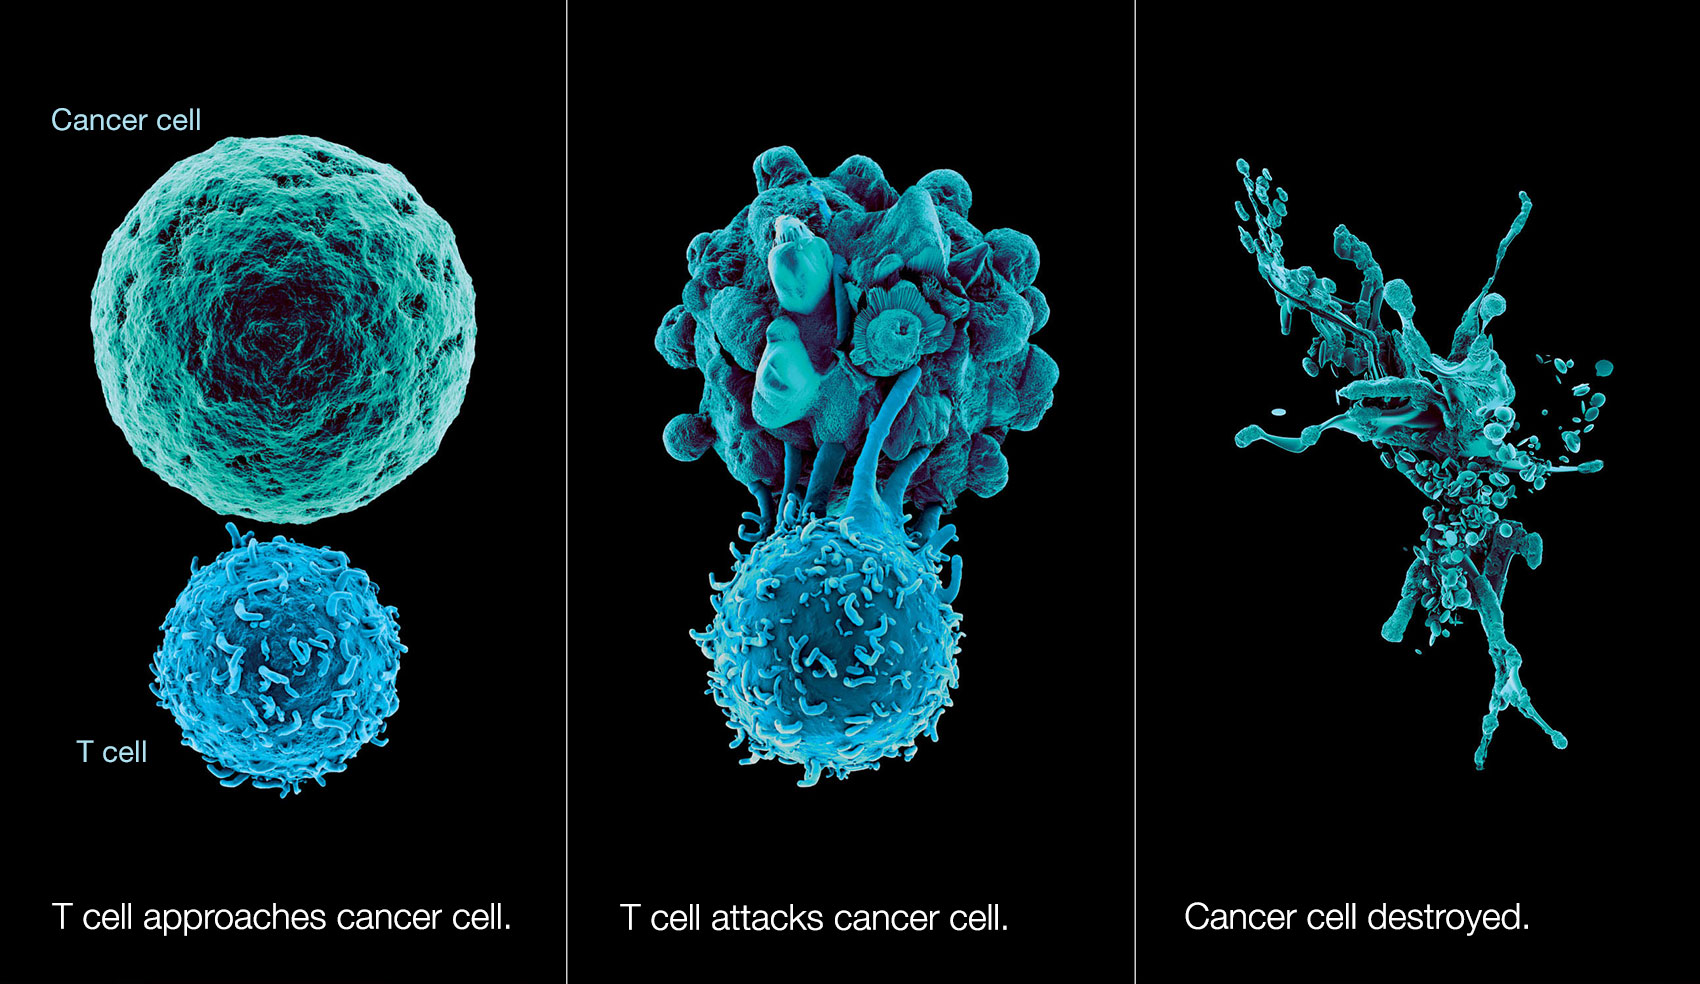
\includegraphics[width=0.85\textwidth]{img/neoantigen/tcell}
		\caption{Ejemplo de como una célula T destruye células del cancer \cite{nortshore2022}.}
	\end{figure}		
\end{frame}
%-------------------------------------------------------
%-------------------------------------------------------

%-------------------------------------------------------
%-------------------------------------------------------
\begin{frame}{Inmunoterapia del Cáncer}{Neo antígenos}		
	\begin{block}{}
		Es una \textbf{proteína} que se forma en las células de Cáncer cuando ocurre mutaciones en el DNA, cumplen un rol importante al \textbf{estimular una respuesta inmune} \cite{NCIdictionary2022, borden2022cancer}.
	\end{block} 
	\begin{block}{}
		En la actualidad hay varios métodos para detectar a predecir neo antígenos, pero \textbf{solo una pequeña cantidad de ellos} logran estimular al sistema inmune \cite{chen2021challenges, hao2021improvement}.
	\end{block}
\end{frame}
%-------------------------------------------------------
%-------------------------------------------------------

%-------------------------------------------------------
%-------------------------------------------------------
\begin{frame}{MHC-I}{}		
	\begin{figure}[H]
		\centering
		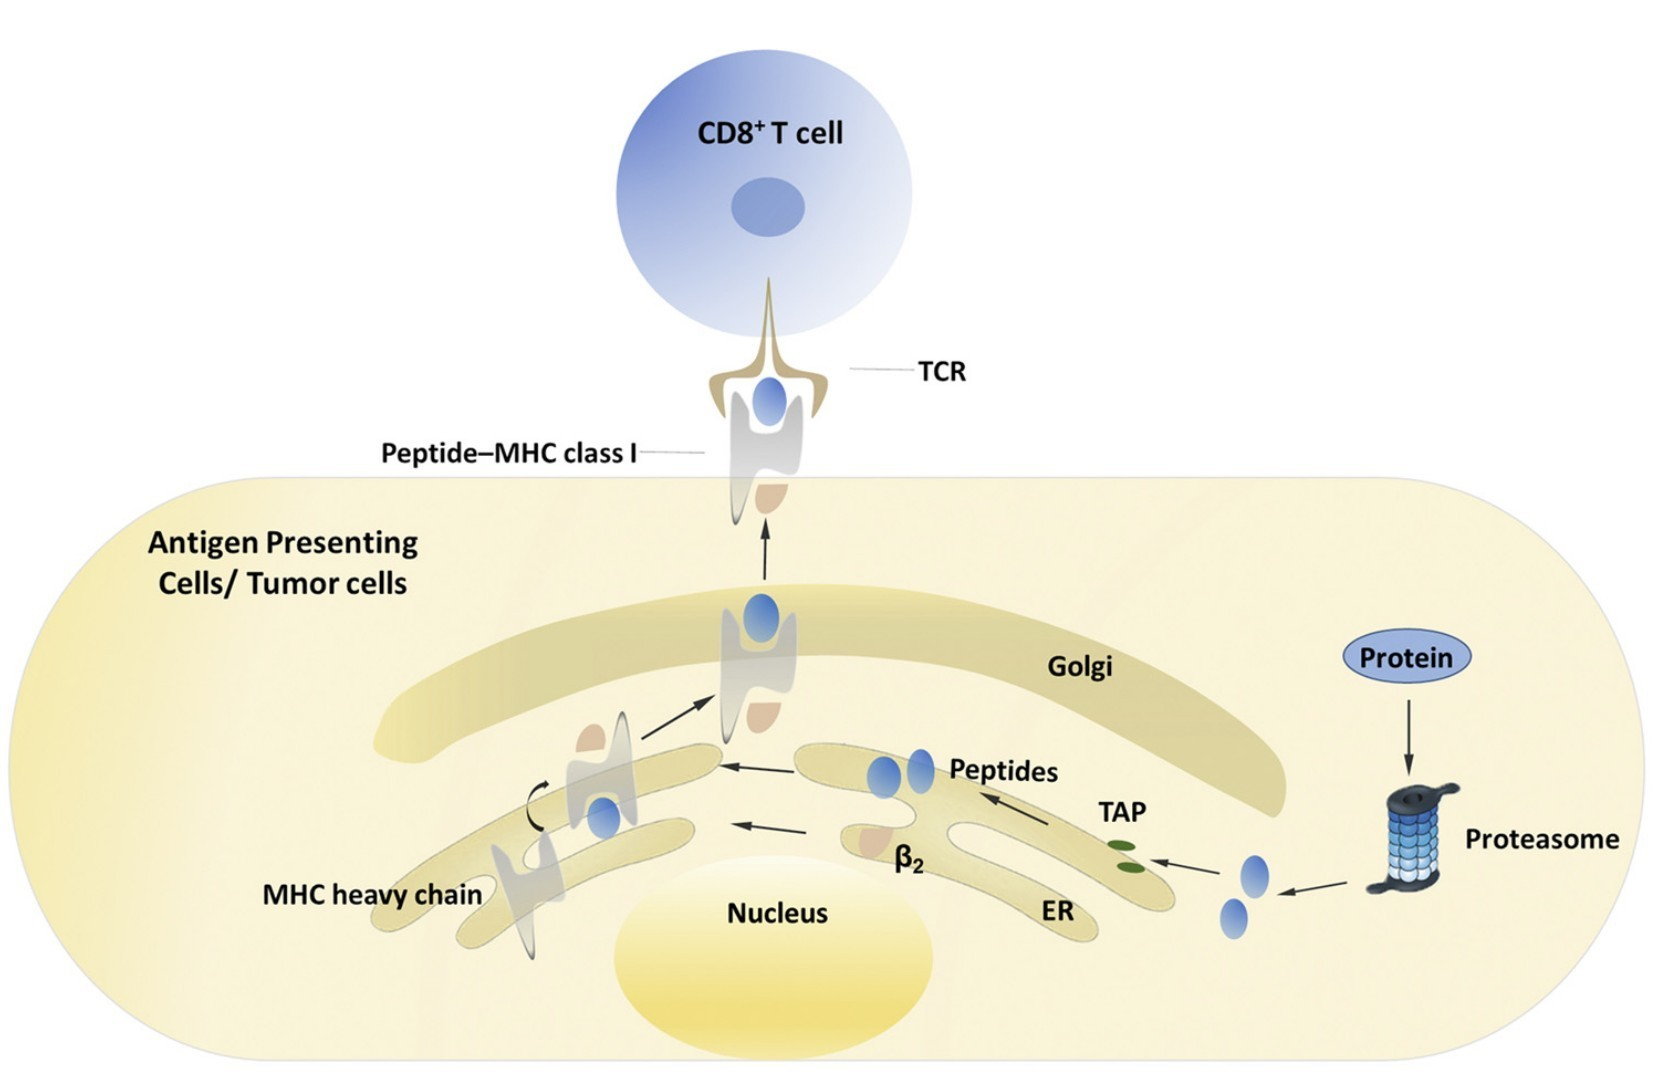
\includegraphics[width=0.9\textwidth]{img/neoantigen/mhc1.jpg}
		\caption{Presentación de antígenos por MHC-I. Fuente: \cite{zhang2019application}}
		\label{fig:mhc1}
	\end{figure}	
\end{frame}
%-------------------------------------------------------
%-------------------------------------------------------

%-------------------------------------------------------
%-------------------------------------------------------
\begin{frame}{MHC-II}{}		
	\begin{figure}[H]
		\centering
		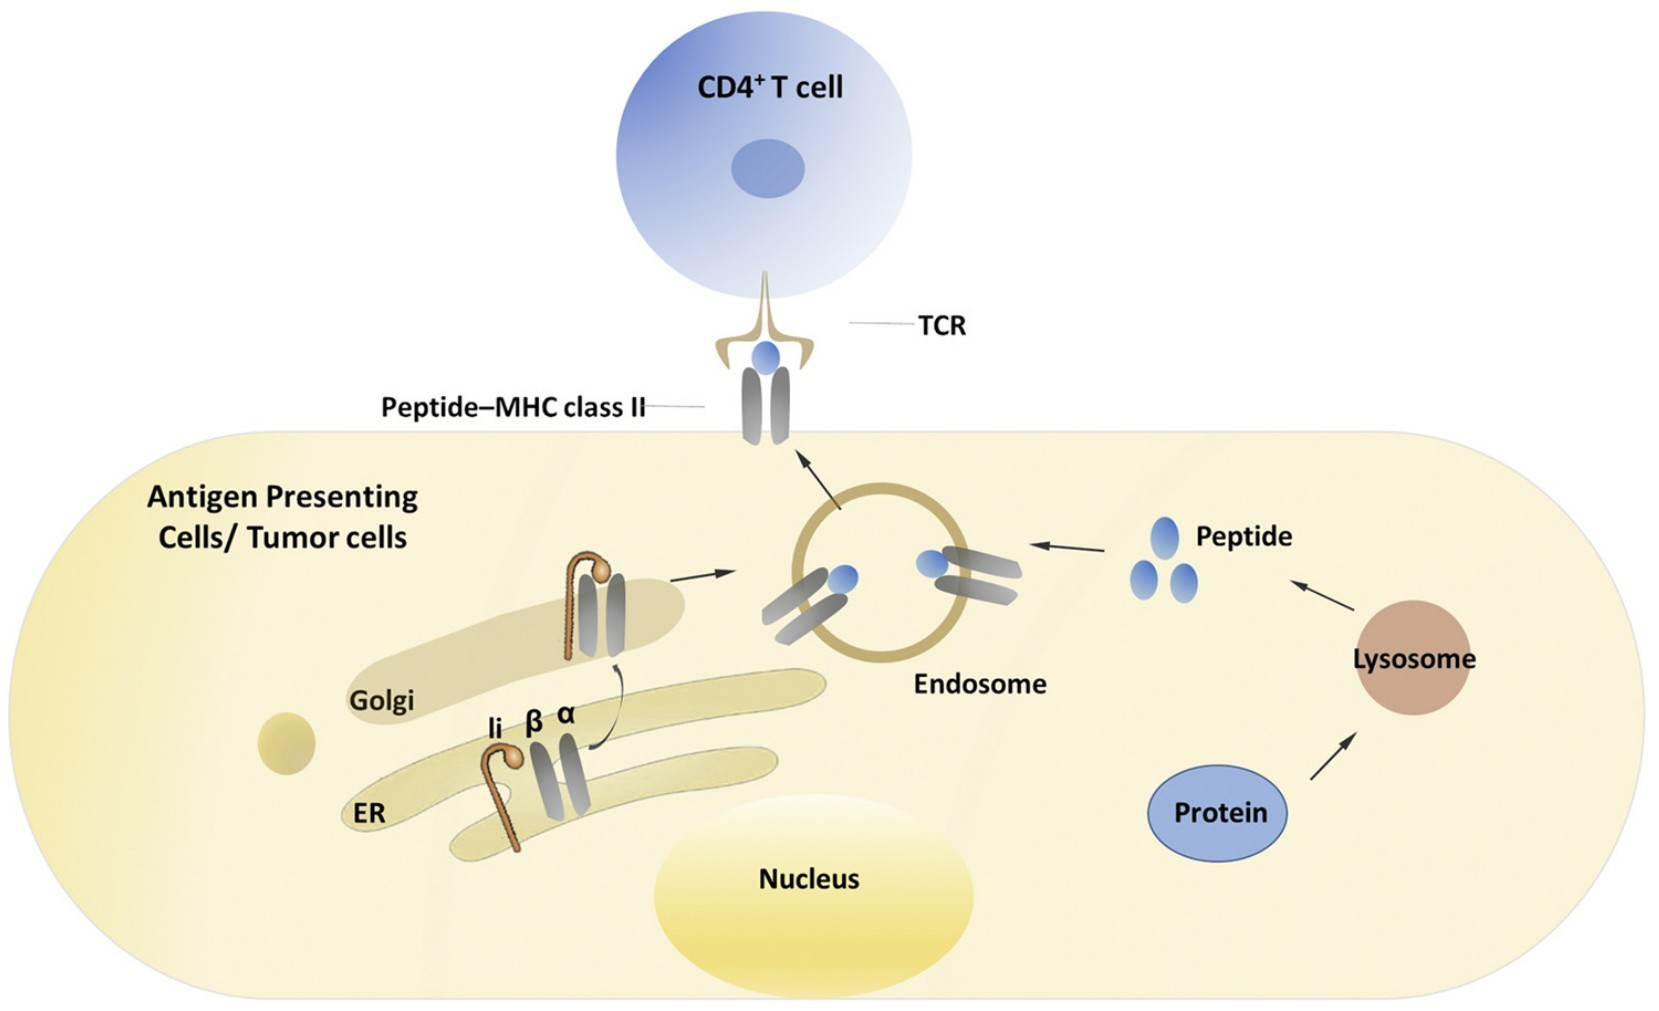
\includegraphics[width=0.9\textwidth]{img/neoantigen/mhc2.jpg}
		\caption{Presentación de antígenos por MHC-II. Fuente: \cite{zhang2019application}}
		\label{fig:mhc2}
	\end{figure}	
\end{frame}
%-------------------------------------------------------
%-------------------------------------------------------

%-------------------------------------------------------
%-------------------------------------------------------
\begin{frame}{Inmunoterapia del Cáncer}{Generación de vacunas}	
	\begin{figure}
		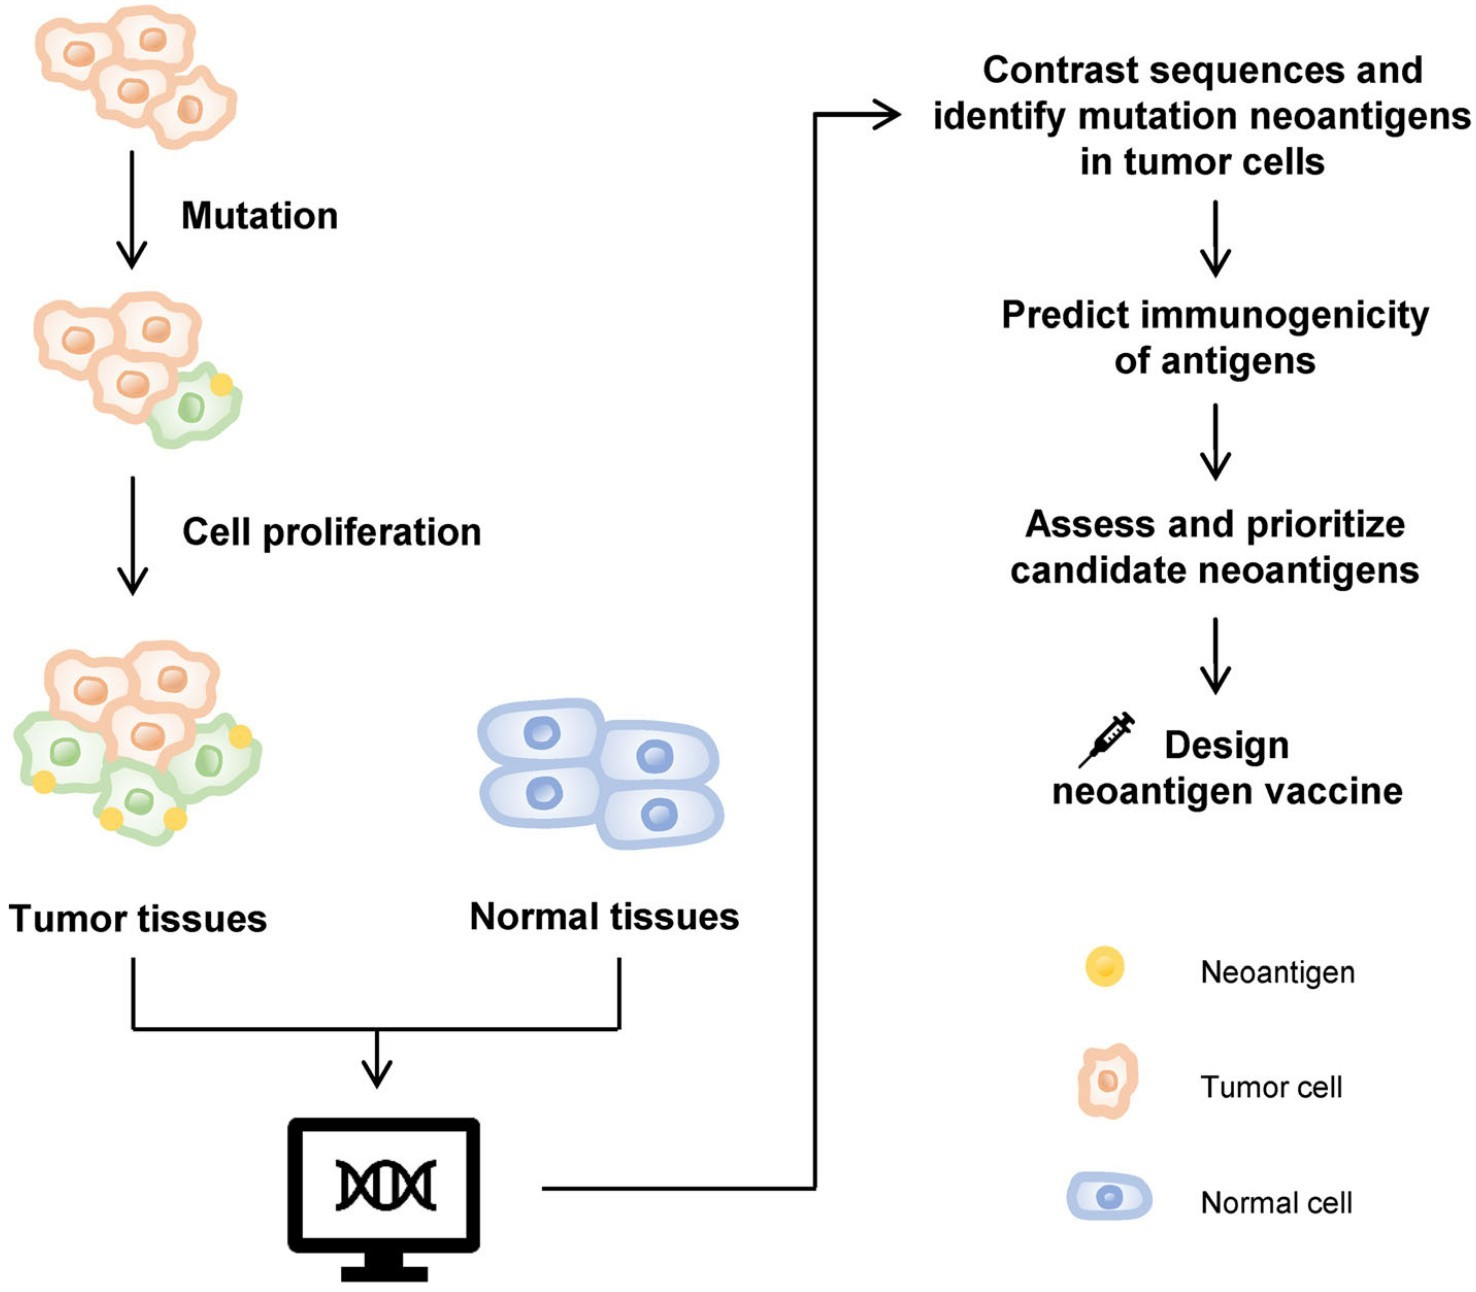
\includegraphics[width=0.6\textwidth]{img/neoantigen/process}
		\caption{Proceso para la generación de vacunas personalizadas \cite{peng2019neoantigen}.}
	\end{figure}		
\end{frame}
%-------------------------------------------------------
%-------------------------------------------------------


%%%%%%%%%%%%%%%%%%%%%%%%%%%%%%%%%%%%%%%%%%%%%%%%%%%%%%%%%%%%%%%%%%%%%%%%%%%%%%%%%%%%%%%%%%%%%%%%%%%%%%%%%%%%%%%%
%%%%%%%%%%%%%%%%%%%%%%%%%%%%%%%%%%%%%%%%%%%%%%%%%%%%%%%%%%%%%%%%%%%%%%%%%%%%%%%%%%%%%%%%%%%%%%%%%%%%%%%%%%%%%%%%
%%%%%%%%%%%%%%%%%%%%%%%%%%%%%%%%%%%%%%%%%%%%%%%%%%%%%%%%%%%%%%%%%%%%%%%%%%%%%%%%%%%%%%%%%%%%%%%%%%%%%%%%%%%%%%%%
\section{Problema y Objetivos}
%%%%%%%%%%%%%%%%%%%%%%%%%%%%%%%%%%%%%%%%%%%%%%%%%%%%%%%%%%%%%%%%%%%%%%%%%%%%%%%%%%%%%%%%%%%%%%%%%%%%%%%%%%%%%%%%
%%%%%%%%%%%%%%%%%%%%%%%%%%%%%%%%%%%%%%%%%%%%%%%%%%%%%%%%%%%%%%%%%%%%%%%%%%%%%%%%%%%%%%%%%%%%%%%%%%%%%%%%%%%%%%%%
%%%%%%%%%%%%%%%%%%%%%%%%%%%%%%%%%%%%%%%%%%%%%%%%%%%%%%%%%%%%%%%%%%%%%%%%%%%%%%%%%%%%%%%%%%%%%%%%%%%%%%%%%%%%%%%%

\subsection{Motivación y Problema}

%-------------------------------------------------------
%-------------------------------------------------------
\begin{frame}{Motivación}{}	

\begin{block}{}
	El cáncer representa el mayor problema de salud mundial, pero lamentablemente los métodos basados en cirugías, radioterapias, quimioterapias tienen baja efectividad \cite{peng2019neoantigen}.
\end{block}	

\begin{block}{}
	La inmunoterapia del cáncer es una alternativa para el desarrollo de vacunas personalizadas, pero este proceso depende de una correcta detección de neo antígenos \cite{de2020neoantigen, peng2019neoantigen}.
\end{block}

\end{frame}
%-------------------------------------------------------
%-------------------------------------------------------



%-------------------------------------------------------
%-------------------------------------------------------
\begin{frame}{Problema}{}
	
\begin{block}{}
	\textbf{Menos del 3\%} de los neoantígenos detectados logran activar a las células T (sistema inmune) \cite{de2020neoantigen}. 
\end{block}
	
\end{frame}
%-------------------------------------------------------
%-------------------------------------------------------

\subsection{Objetivo}

%-------------------------------------------------------
%-------------------------------------------------------
\begin{frame}{Objetivos}{Objetivo general}	
	\begin{block}{Objetivo general}
		Desarrollar un método basado en \textit{deep learning} que mejore el acierto de la detección de neo antígenos.
	\end{block}	
\end{frame}
%-------------------------------------------------------
%-------------------------------------------------------

%-------------------------------------------------------
%-------------------------------------------------------
\begin{frame}{Objetivos}{}	
	\begin{figure}
		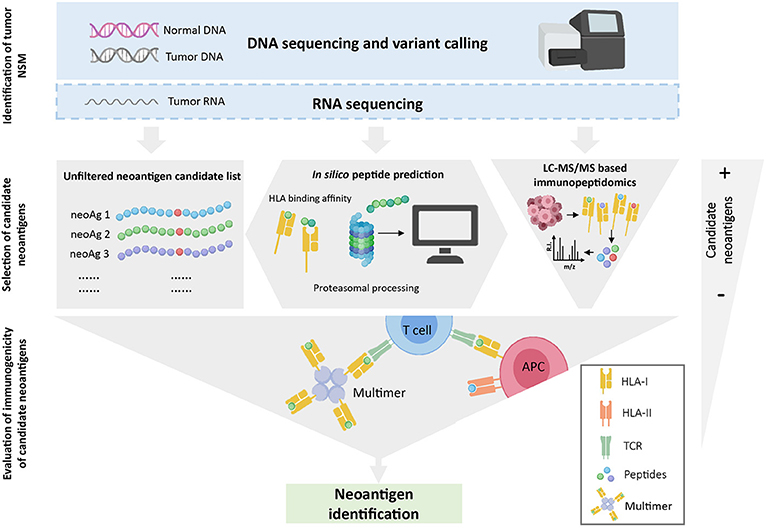
\includegraphics[width=0.97\textwidth]{img/neoantigen/pipeline_neoantigen}
		%\caption{Proceso de la detección de neo antígenos \cite{garcia2019determinants}.}
	\end{figure}
\end{frame}
%-------------------------------------------------------
%-------------------------------------------------------


%%%%%%%%%%%%%%%%%%%%%%%%%%%%%%%%%%%%%%%%%%%%%%%%%%%%%%%%%%%%%%%%%%%%%%%%%%%%%%%%%%%%%%%%%%%%%%%%%%%%%%%%%%%%%%%%
%%%%%%%%%%%%%%%%%%%%%%%%%%%%%%%%%%%%%%%%%%%%%%%%%%%%%%%%%%%%%%%%%%%%%%%%%%%%%%%%%%%%%%
\section{Estado del arte}
%%%%%%%%%%%%%%%%%%%%%%%%%%%%%%%%%%%%%%%%%%%%%%%%%%%%%%%%%%%%%%%%%%%%%%%%%%%%%%%%%%%%%%%%%%%%%%%%%%%%%%%%%%%%%%%%
%%%%%%%%%%%%%%%%%%%%%%%%%%%%%%%%%%%%%%%%%%%%%%%%%%%%%%%%%%%%%%%%%%%%%%%%%%%%%%%%%%%%%%



%-------------------------------------------------------
%-------------------------------------------------------
\begin{frame}{Estado del arte}{\textit{Pipelines}}
	\begin{table}[]
		\setlength{\tabcolsep}{0.5em} % for the horizontal padding
		{\renewcommand{\arraystretch}{1.4}% for the vertical padding
			\begin{tabular}{lp{5cm}l}
				\textbf{Año} & \textbf{Nombre} & \textbf{Referencia}  \\ \hline
				2020  & ProGeo-neo     &\cite{li2020progeo}   \\
				2020  & INeo-Epp     &\cite{wang2020ineo}   \\
				2020  & pVACtools     &\cite{hundal2020pvactools}   \\
				2019  & NeoPredPipe     &\cite{schenck2019neopredpipe}   \\
				2019  & DeepHLApan     &\cite{wu2019deephlapan}   \\
				2019  & ScanNeo     &\cite{wang2019scanneo}   \\     
				2017  & CloudNeo     &\cite{bais2017cloudneo}   \\     
				... & ... & ... \\              
			\end{tabular}
		}
	\end{table}
\end{frame}
%-------------------------------------------------------
%-------------------------------------------------------

%-------------------------------------------------------
%-------------------------------------------------------
\begin{frame}{Estado del arte}{\textit{Peptide-MHC binding}}
	\begin{table}[]
		\setlength{\tabcolsep}{0.5em} % for the horizontal padding
		{\renewcommand{\arraystretch}{1.4}% for the vertical padding
			\begin{tabular}{llp{4cm}l}
				\textbf{Año} & \textbf{Nombre} & \textbf{Modelo} & \textbf{Referencia}  \\ \hline
				2022  & AEM  & Transformer   &\cite{hashemi2022improved}   \\
				2021  & \textbf{BERTMHC}  & Transformer   &\cite{cheng2021bertmhc}   \\
				2021  & \textbf{APPM}  & 3 CNN   &\cite{hao2021improvement}   \\
				2020  & NetMHCpan4.1  & ANN   &\cite{reynisson2020netmhcpan}   \\
				2020  & MHCflurry2.0  & ANN   &\cite{o2020mhcflurry}   \\
				2020  & MHCnuggets  & ANN   &\cite{shao2020high}   \\
         	    2019  & PUFFIN  & ANN   &\cite{zeng2019quantification}   \\
         	    ..  & ...  & ...   &...   \\	            
			\end{tabular}
		}
	\end{table}
\end{frame}
%-------------------------------------------------------
%-------------------------------------------------------

%%%%%%%%%%%%%%%%%%%%%%%%%%%%%%%%%%%%%%%%%%%%%%%%%%%%%%%%%%%%%%%%%%%%%%%%%%%%%%%%%%%%%%%%%%%%%%%%%%%%%%%%%%%%%%%%
%%%%%%%%%%%%%%%%%%%%%%%%%%%%%%%%%%%%%%%%%%%%%%%%%%%%%%%%%%%%%%%%%%%%%%%%%%%%%%%%%%%%%%
\section{Propuesta}
%%%%%%%%%%%%%%%%%%%%%%%%%%%%%%%%%%%%%%%%%%%%%%%%%%%%%%%%%%%%%%%%%%%%%%%%%%%%%%%%%%%%%%%%%%%%%%%%%%%%%%%%%%%%%%%%
%%%%%%%%%%%%%%%%%%%%%%%%%%%%%%%%%%%%%%%%%%%%%%%%%%%%%%%%%%%%%%%%%%%%%%%%%%%%%%%%%%%%%%



%-------------------------------------------------------
%-------------------------------------------------------
\begin{frame}{Propuesta}{}

		La propuesta se basa el los modelos BERTMHC \cite{cheng2021bertmhc} y APPM \cite{hao2021improvement}.
		


	\vspace{0.5cm}
	\begin{figure}
		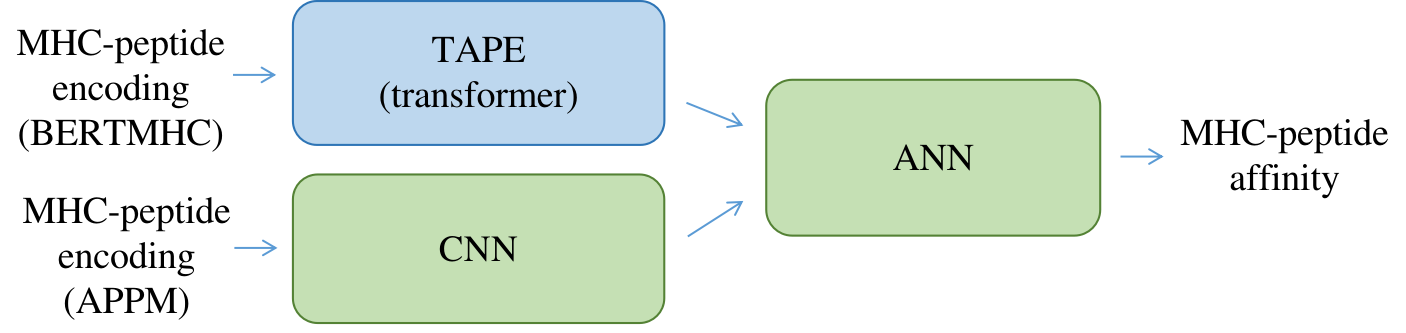
\includegraphics[width=0.97\textwidth]{img/neoantigen/proposal2}
		\caption{Modelo propuesto para la predicción del enlace péptido y MHC.}
	\end{figure}
\end{frame}
%-------------------------------------------------------
%-------------------------------------------------------

%-------------------------------------------------------
%-------------------------------------------------------
\begin{frame}{Propuesta}{BERTMHC}	
	\begin{figure}
		\centering
		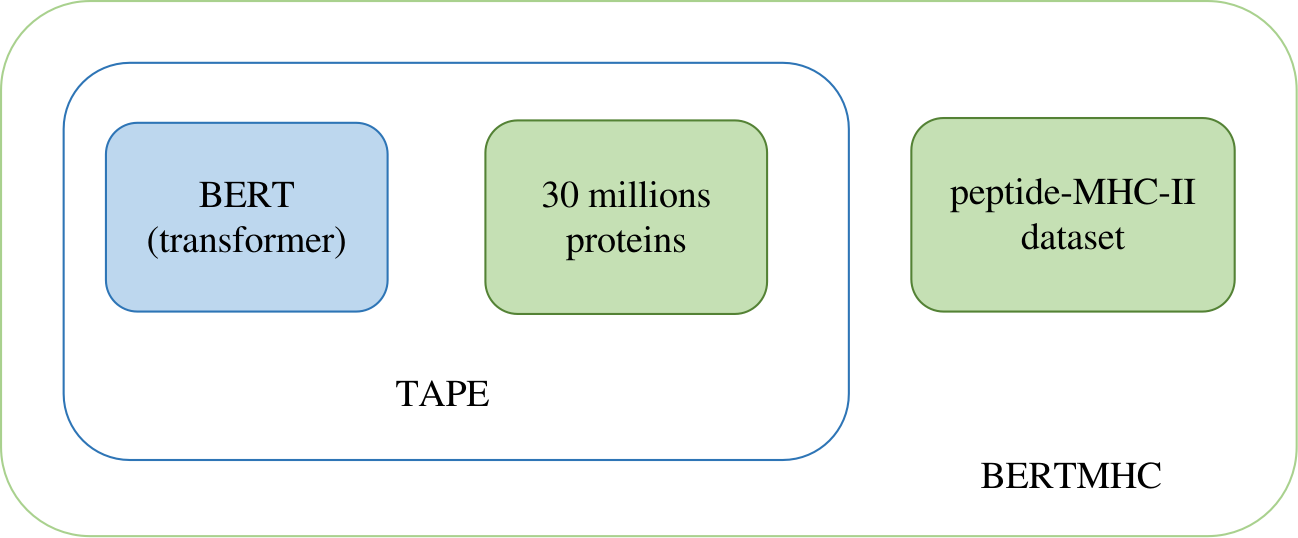
\includegraphics[width=0.9\textwidth]{img/neoantigen/bertmhc}	
		\caption{BERTMHC.}
	\end{figure}
\end{frame}
%-------------------------------------------------------
%-------------------------------------------------------

%-------------------------------------------------------
%-------------------------------------------------------
\begin{frame}{Propuesta}{APPM}	
	\begin{figure}
		\centering
		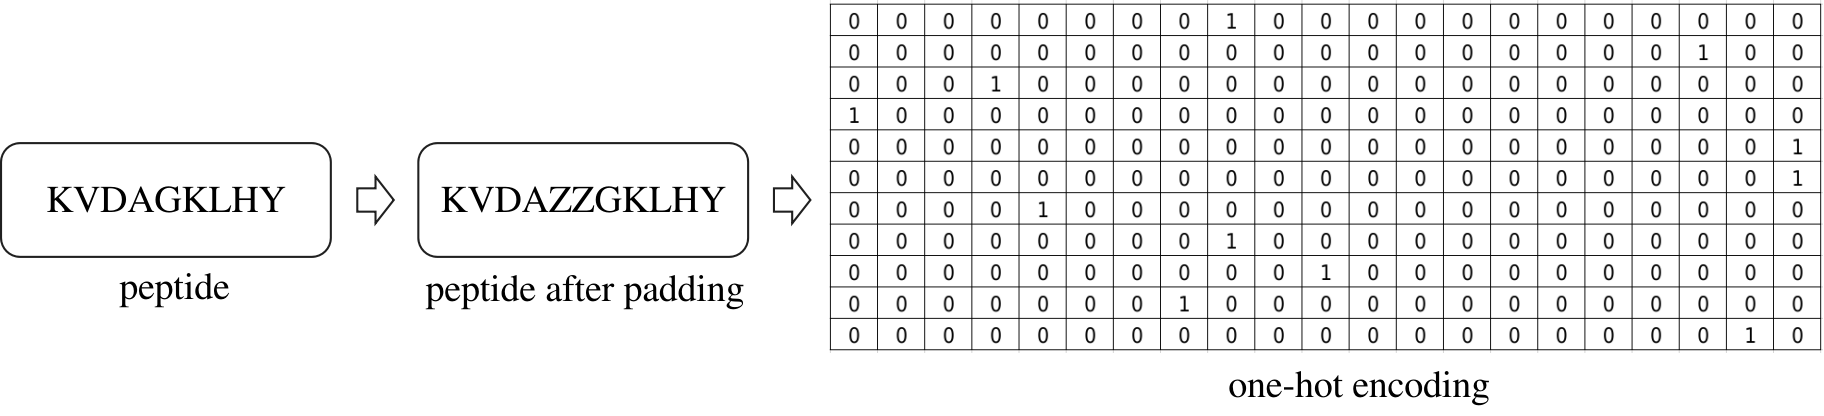
\includegraphics[width=\textwidth]{img/neoantigen/descriptor}	
		\caption{Proceso para obtener una matriz (imagen) a partir de un péptido (APPM).}
		\label{fig:descriptor}
	\end{figure}
\end{frame}
%-------------------------------------------------------
%-------------------------------------------------------

%%%%%%%%%%%%%%%%%%%%%%%%%%%%%%%%%%%%%%%%%%%%%%%%%%%%%%%%%%%%%%%%%%%%%%%%%%%%%%%%%%%%%%%%%%%%%%%%%%%%%%%%%%%%%%%%
%%%%%%%%%%%%%%%%%%%%%%%%%%%%%%%%%%%%%%%%%%%%%%%%%%%%%%%%%%%%%%%%%%%%%%%%%%%%%%%%%%%%%%
\section{Resultados}
%%%%%%%%%%%%%%%%%%%%%%%%%%%%%%%%%%%%%%%%%%%%%%%%%%%%%%%%%%%%%%%%%%%%%%%%%%%%%%%%%%%%%%%%%%%%%%%%%%%%%%%%%%%%%%%%
%%%%%%%%%%%%%%%%%%%%%%%%%%%%%%%%%%%%%%%%%%%%%%%%%%%%%%%%%%%%%%%%%%%%%%%%%%%%%%%%%%%%%%

%-------------------------------------------------------
%-------------------------------------------------------
\begin{frame}{Base de datos}{}
	\begin{table}[h]
		\centering
		\caption{Cantidad de muestras por tipo de \textit{allele}.}
		\label{tab:db}
		\setlength{\tabcolsep}{0.8em} % for the horizontal padding
		{\renewcommand{\arraystretch}{1.3}% for the vertical padding
			\begin{tabular}{ccccc}
				\hline
				\textit{\textbf{Alleles}} & \textbf{Label = 1} & \textbf{Label = 0} & \textbf{Train}  & \textbf{Test}  \\ \hline
				A*01:01                   & 3398               & 48700              & 45498  & 6600  \\ 
				A*02:01                   & 6779               & 165342             & 160921 & 11200 \\ 
				A*02:03                   & 1780               & 116299             & 107879 & 10200 \\ 
				A*31:01                   & 1879               & 45918              & 41597  & 6200  \\ 
				B*44:02                   & 1525               & 44760              & 40085  & 6200  \\ 
				B*44:03                   & 1487               & 39482              & 34769  & 6200  \\ 
				MHC-II alleles            & 1917               & 496                & 1533  & 384  \\ 
			\end{tabular}
		}
	\end{table}
\end{frame}
%-------------------------------------------------------
%-------------------------------------------------------

%-------------------------------------------------------
%-------------------------------------------------------
\begin{frame}{Resultados}{}
\begin{table}[]
	\centering
	\caption{Resultados obtenidos en cada base de datos. }
	\label{tab:results}
	\setlength{\tabcolsep}{0.8em} % for the horizontal padding
	{\renewcommand{\arraystretch}{1.3}% for the vertical padding
		\begin{tabular}{lllll}
			\hline
			\textit{\textbf{Allele}} & \textit{\textbf{Accuracy}} & \textit{\textbf{F1 score}} & \textit{\textbf{Precision}} & \textit{\textbf{Recall}} \\
			\hline
			A*01:01                  & 0.978                      & 0.917                      & 0.982                       & 0.887                    \\
			A*0201                   & 0.962                      & 0.956                      & 0.965                       & 0.948                    \\
			A*02:03                  & 0.992                      & 0.979                      & 0.994                       & 0.969                    \\
			A*31:01                  & 0.980                      & 0.968                      & 0.989                       & 0.951                    \\
			B*44:02                  & 0.991                      & 0.981                      & 0.968                       & 0.997                    \\
			B*44:03                  & 0.992                      & 0.987                      & 0.995                       & 0.980                   
		\end{tabular}
	}
\end{table}
\end{frame}
%-------------------------------------------------------
%-------------------------------------------------------

%-------------------------------------------------------
%-------------------------------------------------------
\begin{frame}{Resultados}{}
	\begin{table}[h]
		\centering
		\caption{AUC entre la propuesta, BERTMHC, NetMHCpan3.2, PUFFIN y MHCnuggets.}
		\setlength{\tabcolsep}{0.8em} % for the horizontal padding
		{\renewcommand{\arraystretch}{1.3}% for the vertical padding
			\begin{tabular}{lc}
				\hline
				\textbf{Modelo} & \textbf{AUC} \\ \hline
				Propuesta & 0.73\\
				BERTMHC & 0.72\\
				NetMHCpan3 & 0.68\\
				PUFFIN & 0.69\\
				MHCnuggets & 0.58\\
			\end{tabular}
		}
	\end{table}
\end{frame}
%-------------------------------------------------------
%-------------------------------------------------------


%%%%%%%%%%%%%%%%%%%%%%%%%%%%%%%%%%%%%%%%%%%%%%%%%%%%%%%%%%%%%%%%%%%%%%%%%%%%%%%%%%%%%%%%%%%%%%%%%%%%%%%%%%%%%%%%
%%%%%%%%%%%%%%%%%%%%%%%%%%%%%%%%%%%%%%%%%%%%%%%%%%%%%%%%%%%%%%%%%%%%%%%%%%%%%%%%%%%%%%
\section{Conclusiones}
%%%%%%%%%%%%%%%%%%%%%%%%%%%%%%%%%%%%%%%%%%%%%%%%%%%%%%%%%%%%%%%%%%%%%%%%%%%%%%%%%%%%%%%%%%%%%%%%%%%%%%%%%%%%%%%%
%%%%%%%%%%%%%%%%%%%%%%%%%%%%%%%%%%%%%%%%%%%%%%%%%%%%%%%%%%%%%%%%%%%%%%%%%%%%%%%%%%%%%%


%-------------------------------------------------------
%-------------------------------------------------------
\begin{frame}{Conclusiones}{}
	\begin{block}{}
		En esta investigación se propuso el uso de un modelo \textit{transformer} ya entrenado con una base de datos de 30 millones de proteínas. Luego, esta red fue conectada de forma paralela con una red CNN.
	\end{block}
	
	\begin{block}{}
		El uso de \textit{transfer learning} es una buena opción para suplir la falta de muestras en ciertos problemas y reducir el tiempo de entrenamiento.		
	\end{block}

	\begin{block}{}
		La propuesta llego a mejorar los mejores métodos de detección de afinidad entre un péptido y una proteína MHC-II. Como trabajo futuro, se planteará la misma propuesta para proteínas MHC-I.	
	\end{block}

	\begin{block}{}
		Predecir la afinidad entre un péptido y una proteína MHC, es uno de los paso mas importantes par calificar al péptido como un neo antígeno, capaz de generar una respuesta inmunitaría.
	\end{block}
\end{frame}
%-------------------------------------------------------
%-------------------------------------------------------

%%%%%%%%%%%%%%%%%%%%%%%%%%%%%%%%%%%%%%%%%%%%%%%%%%%%%%%%%%%%%%%%%%%%%%%%%%%%%%%%%%%%%%%%%%%%%%%%%%%%%%%%%%%%%%%%
%%%%%%%%%%%%%%%%%%%%%%%%%%%%%%%%%%%%%%%%%%%%%%%%%%%%%%%%%%%%%%%%%%%%%%%%%%%%%%%%%%%%%%
\section{Trabajos futuros}
%%%%%%%%%%%%%%%%%%%%%%%%%%%%%%%%%%%%%%%%%%%%%%%%%%%%%%%%%%%%%%%%%%%%%%%%%%%%%%%%%%%%%%%%%%%%%%%%%%%%%%%%%%%%%%%%
%%%%%%%%%%%%%%%%%%%%%%%%%%%%%%%%%%%%%%%%%%%%%%%%%%%%%%%%%%%%%%%%%%%%%%%%%%%%%%%%%%%%%%


%-------------------------------------------------------
%-------------------------------------------------------
\begin{frame}{Trabajos futuros}{}
	\begin{block}{}
		Recientemente un trabajo \cite{hashemi2022improved} tambien propone el uso de \textit{transfer learning} pero de un modelo pre-entrenado con 250 millones de proteínas. Entonces, se plantea utilizar la misma red, aumentar la cantidad de muestras y evaluar los resultados.
	\end{block}
	
	\begin{block}{}
		Actualmente se cuenta con una base de datos de proteínas MHC \cite{e2019phla3d}, entonces utilizando AlphaFold de Google, se plantea predecir la estructura de varios péptidos y analizar el enlace péptido-MHC desde un punto de vista de la computación gráfica.	
	\end{block}
	
	
\end{frame}
%-------------------------------------------------------
%-------------------------------------------------------

%-------------------------------------------------------
%-------------------------------------------------------
\begin{frame}[allowframebreaks]
	\frametitle{References}
	%\bibliographystyle{amsalpha}
	\bibliographystyle{IEEEtran}
	\bibliography{Bibliography.bib}
\end{frame}
%-------------------------------------------------------
%-------------------------------------------------------

%-------------------------------------------------------
%-------------------------------------------------------
\if\mycmd1 % MY THEME
\1{
	{\1
		\begin{frame}[plain,noframenumbering]
			%\finalpage{Thank you}
			\begin{figure}[]
				\centering
				
\includegraphics[width=\textwidth,height=0.7\textheight,keepaspectratio]{img/question.png}
				%\label{img:mot2}
				%\caption{Image example in 2 gray levels.}
			\end{figure}
	\end{frame}}
	\else % CS THEME
	\begin{frame}{Questions?}
		\begin{figure}[]
			\centering
			
\includegraphics[width=\textwidth,height=0.7\textheight,keepaspectratio]{img/question.png}
			%\label{img:mot2}
			%\caption{Image example in 2 gray levels.}
		\end{figure}
		
	\end{frame}
	\fi
	%-------------------------------------------------------
	%-------------------------------------------------------
	

\end{document}